\documentclass[12pt,preprint]{aastex631}

\newcommand{\vdag}{(v)^\dagger}
\newcommand\aastex{AAS\TeX}
\newcommand\latex{La\TeX}

\graphicspath{{./}{figures/}}
\usepackage{graphicx}
\usepackage{gensymb}
\usepackage{amsmath}
\usepackage{comment}
\usepackage{amssymb}

\bibliographystyle{plain}


\def\Msun{M_\odot}                                % solar masses
\def\deg{^\circ}
\def\aa{\buildrel _{\circ} \over {\mathrm{A}}}
\newcommand{\Alfven}{Alfv$\acute{\rm e}$n~}
\newcommand{\Alfvenic}{Alfv$\acute{e}$nic~}


\begin{comment}
% FIGSET-MACROS-BEGIN
\newcommand{\noprint}[1]{}
\newcommand{\figsetstart}{{\bf Fig. Set} }
\newcommand{\figsetend}{}
\newcommand{\figsetgrpstart}{}
\newcommand{\figsetgrpend}{}
\newcommand{\figsetnum}[1]{{\bf #1.}}
\newcommand{\figsettitle}[1]{ {\bf #1} }
\newcommand{\figsetgrpnum}[1]{\noprint{#1}}
\newcommand{\figsetgrptitle}[1]{\noprint{#1}}
\newcommand{\figsetplot}[1]{\noprint{#1}}
\newcommand{\figsetgrpnote}[1]{\noprint{#1}}
% FIGSET-MACROS-END
\end{comment}

%\newcommand\myfontsizeII{\fontsize{6pt}{12pt}\selectfont}

\shortauthors{Reines et al.}

%%%%%%%%%%%%%%%%%%%%%%%%%%%%%%%%%%%%%%%%%%%%%%%%%%%%%%%%%%%%%%%%%%%%%%

\begin{document}

\title{VARIABILITY AND PARAMETER DEPENDENCE OF HARD X-RAY OBSCURATION AROUND SUPERMASSIVE BLACK HOLES IN ACTIVE GALAXIES
\footnote{Created: June, 7, 2022}}

\author[0000-0002-0786-7307]{Abraham J. Reines}
\author[0000-0002-0786-7307]{Keigo Fukumura}
\affiliation{Physics and Astronomy Department at JMU \\
901 Carrier Dr, Harrisonburg, VA 22807 \\
Harrisonburg, VA 22801, USA}

\begin{abstract}

We investigate hard X-ray obscuration of Active Galactic Nuclei (AGN) by considering photoionization processes for a number of simulated accretion-disk winds in our magnetohydrodynamic (MHD) framework. To follow up our earlier work on calculating synthetic AGN obscuration functions, we are motivated in this work to expand our examination of the dependences of obscuration on individual parameters associated with MHD wind and coronal X-ray such as: X-ray luminosity $L_{\rm ion}$, photon index $\Gamma$, density of the wind $n_o$ and its radial gradient $p$ where $n$ $\propto$ $n_o r^{-p}$.  We find that AGN appear to undergo a relatively drastic transition from more obscured state (e.g. $N_H \gtrsim 10^{22}$ cm$^{-2}$) to unobscured state (i.e. $N_H \lesssim 10^{22}$ cm$^{-2}$) as $p$ approaches to $\sim$ 1.1 in these calculations. In the current formalism, luminosity is linearly coupled to wind density (i.e. $L_X \propto n_o$), and our calculations also indicate AGN become more obscured at higher luminosity. We further discuss the plausibility of the current model in comparison with observations.

\end{abstract}

\keywords{AGN Host Galaxies  --- X-ray Active Galactic Nuclei  --- Radiative Magnetohydrodynamics}

%%%%% INTRODUCTION %%%%%

\section{Introduction}

In our earlier note \citep{Reines22}, we report a general feature of the absorption function predicted by our magnetohydrodynamic (MHD) disk-wind model \citep[e.g.][]{F10} in which many AGN are expected to be unobscured at low X-ray luminosity and low wind density. This is partly consistent with data derived from a large number of X-ray surveys \citep[e.g.][]{Ueda03,Buchner15}, while we also note in our predictions some discrepencies in the obscured AGN populations at intermediate luminosity. For example, those observations suggest the obscuration decreases with increasing $L_X$ ignoring a likely dependence on $\Gamma$. In \cite{Reines22}, we were unable to draw a convincing conclusion due to our narrow choice of the parameter ranges in $\Gamma$ and $L_X$.  In this note, therefore, we exploit the model predictions by focusing on broader parameter ranges with a special interest in exploring the exclusive dependences on X-ray property (i.e. $L_X$ and $\Gamma$) and wind condition (i.e. $n_o$ and $p$) as addressed next.  


%%%%% METHODS %%%%%

\section{Methods}

Our model institutes MHD equations to determine a geometrical structure of magnetized outflows under strong gravity.  Plasma is magnetically lifted away from the BH accretion disk through magnetic field lines.  By numerically solving MHD equations for this extreme magnetosphere environment, we obtain a set of fiducial solutions for disk winds.  To reduce extra degrees of freedom in our model, we fix a given wind morphology throughout the simulations, while considering different wind density structure and radiation field.

By conducting radiative transfer calculations with {\tt xstar} \citep[][]{Kallman01}, we simulate predicted hard X-ray spectra for various sets of the parameters to be fitted with a single power-law model (in $10-50$ keV band), as we constrain the degree of hard X-ray obscuration by obtaining the neutral column density, $N_H$, as a proxy for obscuration.

In the past work, we have shown the fraction of X-ray obscured AGN, described by an absorption function, is directly related to intrinsic X-ray luminosity $L_X$, and wind density normalization $n_o$.  
%This absorption function is expressed using obscuring column density, $N_H$.  \cite{Reines}
%
Extending the earlier effort with a focus on specific model parameters, the present work further explores unique roles of X-ray luminosity $L_X$, wind density $n_o$, radial gradient $p$, and photon index $\Gamma$.  

%We calculate the column density, $N_H$, of outflowing X-ray-absorbing plasma (i.e. ionized winds) to construct a distribution of $N_H$ as functions for each parameter.  

%We conduct radiative transfer process (RTP) calculations to examine these parameter's influence on $N_H$.

To examine the individual influences of $\Gamma$, $n_o$, $L_X$, and $p$, we fix the inclination angle to  $\theta = 45\deg$ throughout these calculations. 

%==
%We first show in Figure~1a (above) the predicted obscuration in terms of $N_H$ as a function of $\Gamma$ for various $L_X$ and $n_0$ assuming $p=1.0$.  Compton thin AGN of weak obscuration suffer from large uncertainty in the bestfit $N_H$ values.  Thus, column density less than $10^{22}$ cm$^{-2}$ is set to $N_H=10^{22}$ cm$^{-2}$.  Figure 1b illustrates how $\Gamma$ influences our $L_X$ simulated results.  Figure 1c illustrates how $N_H$ is influenced as a function of $p$. 


%%%%% CONCLUSIONS AND RESULTS %%%%%

\begin{figure}[h!]% ------------------------------------- Figure~1
\begin{center}$
\begin{array}{cc}
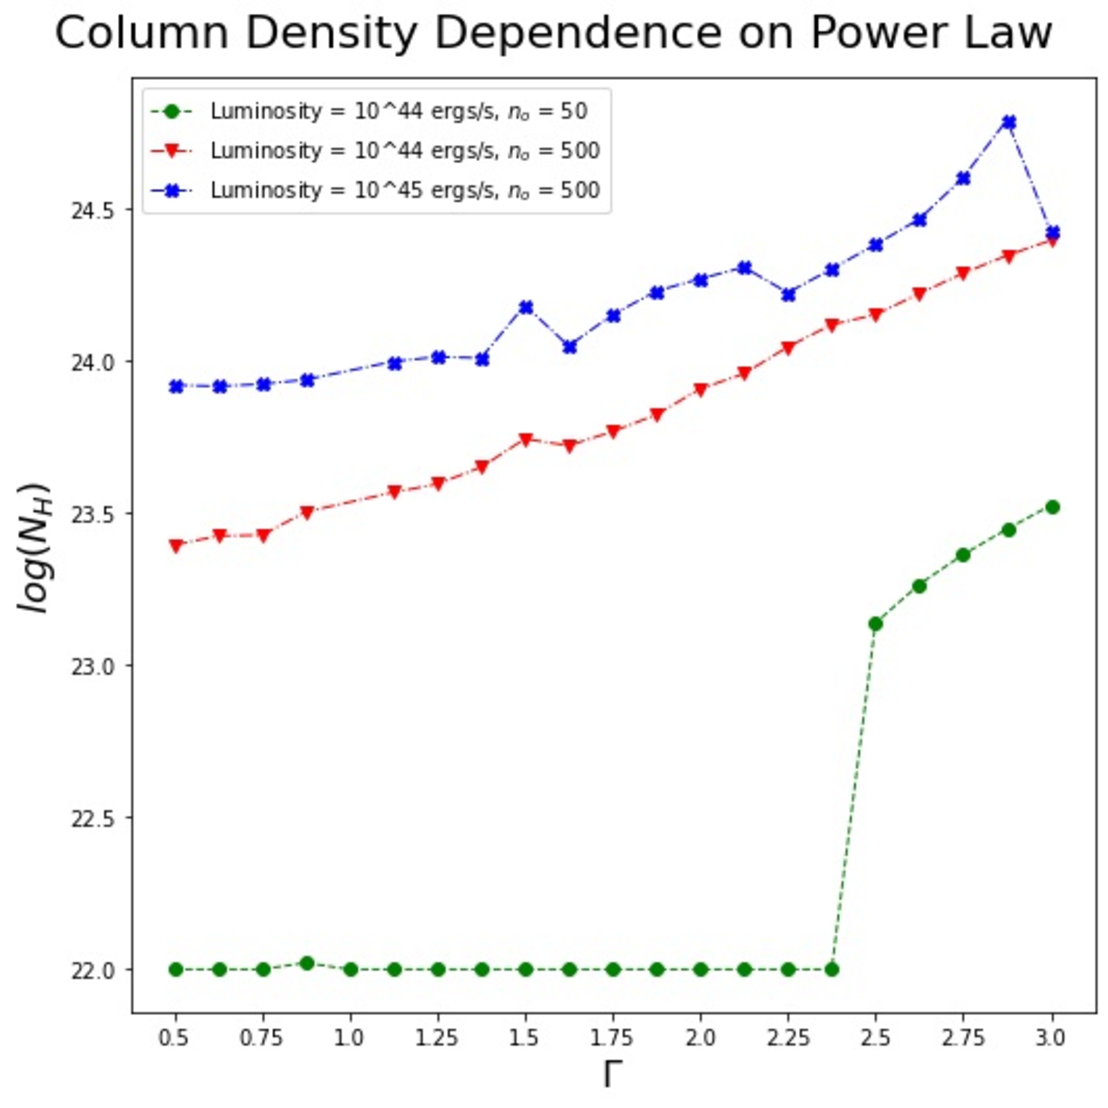
\includegraphics[trim=0in 0in 0in
0in,keepaspectratio=false,width=4.0in,angle=-0,clip=false]{f1_1.pdf}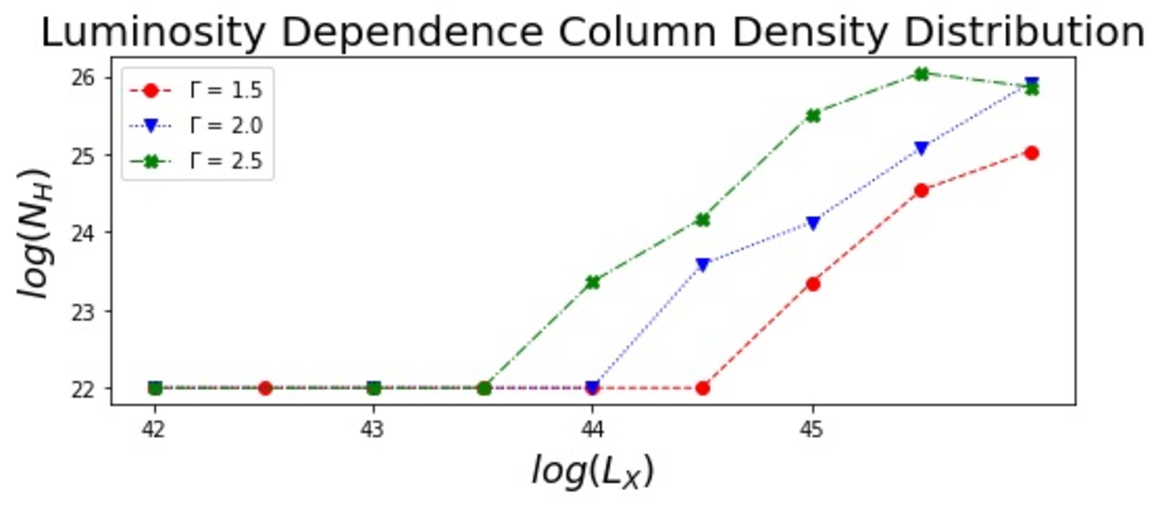
\includegraphics[trim=0in 0in 0in
0in,keepaspectratio=false,width=4.0in,angle=-0,clip=false]{f1_3.pdf}
\\
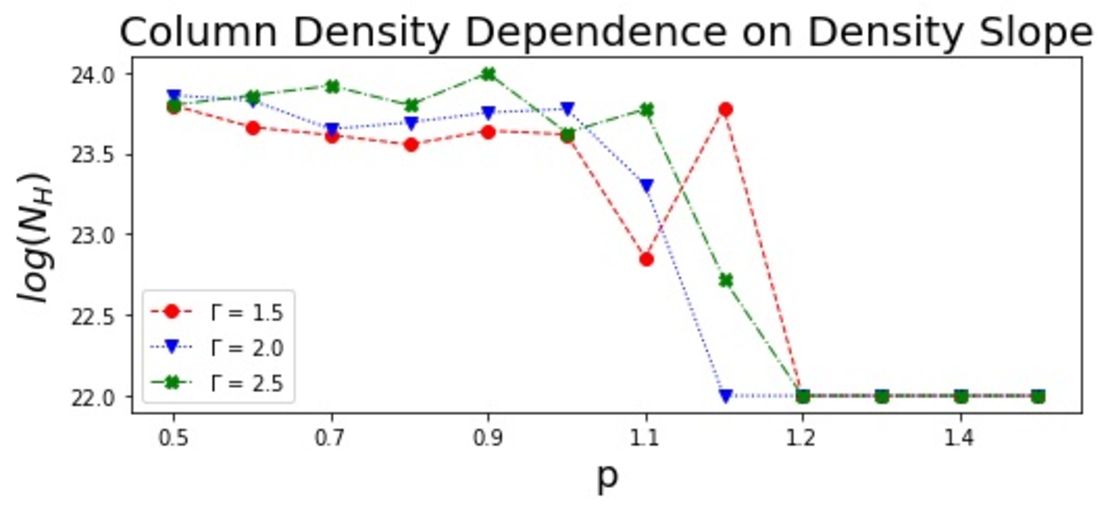
\includegraphics[trim=0in 0in 0in
0in,keepaspectratio=false,width=3.0in,angle=-0,clip=false]{f1_4.pdf}
%\includegraphics[trim=0in 0in 0in
%0in,keepaspectratio=false,width=3.2in,angle=-0,clip=false]{fL5_obs50_windC_Ka+Kb_cont.pdf}
\end{array}$
\end{center}
\caption{Simulated obscuration with $N_H$ for various model parameters. Left: The effect of $\Gamma$ for $L_X=10^{44}$ erg/s and $n_o=50$ (green), $L_X=10^{44}$ erg/s and $n_o=500$ (red) and $L_X=10^{45}$ erg/s and $n_o=500$ (blue) for comparison. Any unconstrained low column, $N_H \le 10^{22}$ cm$^{-2}$, is readjusted to $N_H=10^{22}$ cm$^{-2}$ for simplicity. Upper Right: The effect of $L_X$ for $\Gamma=1.5$ (red), $2$ (blue) and $2.5$ (green) with $p=1.0$ and $\theta=45\deg$. Lower Right: The effect of $p$ for $\Gamma=1.5$ (red), $2$ (blue) and $2.5$ (green) with $p=1.0$ and $\theta=45\deg$.}
\label{fig:f1}
\end{figure}

\section{Conclusions and Results}

Our speculations about obscuration dependence on $L_X$ and $n_o$ hold in this study.  However, our initial findings about $\Gamma$ are somewhat weak. We find in the current work $\Gamma$ exhibits a clear trend when the remaining parameters are held constant; i.e. the softer the X-ray continuum is, the more obscuration.

Figure 1 (Left)  shows the exclusive dependence of obscuration on $\Gamma$ for different sets of $n_o$ and $L_X$. We have found the fraction of obscured AGN increases with increasing $\Gamma$ unless $L_X$ is sufficiently low. The positive correlation between $N_H$ and $\Gamma$ is consistent with how X-ray photons in a harder spectrum (i.e. lower $\Gamma$) generally have, as a matter of fact, more penetrating power through the wind material.  Regardless of $\Gamma$, however, $n_o$ and $L_X$ must be sufficiently low to generate Compton-thin AGN spectra.

The effect of $L_X$ on $N_H$ is given in Figure~1 (Upper Right) for different $\Gamma$. We have coupled $L_X$ and $n_o$ in our physical formalism; i.e. as plasma accretes, X-ray photons are produced and emitted from the corona of a black hole. Therefore, these parameters are inherently correlated, and we have incorporated this into our computational framework. This result appears to be the most contentious in comparison with the observations \citep[e.g.][]{Ueda03}, indicating a physical issue with this coupling assumption in our model. 

In our wind model, a steeper density profile (i.e. larger $p$) forces winds to possess a centrally concentrated material along a line of sight; i.e. a more compact density distribution.  We find $p$ can also affect the extent of obscuration in Figure 1 (Lower Left); i.e. AGN surrounded by a more centrally-concentrated wind (e.g. $p \gtrsim 1.1$) are more visible, while a wind of spatially more extended density profile (e.g. $p \lesssim 1.1$) can effectively obscure AGN. For $p \lesssim 1.1$, AGN with softer spectrum is more obscured as demonstrated earlier. It is interesting to note there exists a critical $p$-value at $p \sim 1.1$ separating obscured AGN from unobscured AGN regardless of $\Gamma$ as if obscuration is suddenly switched off.  We call this an obscuration dichotomy within our wind density profile. Such a hypothesis needs to be explored with more thorough simulations in the future work.   

%%%%% REFERENCES %%%%%
\hfill
  \newpage
  
  %\acknowledge
This work is supported in part by NASA grant, NNH20ZDA001N-ADAP, and through Astrophysics Data Analysis Program and Jeffress Trust Fund.

\begin{thebibliography}{999}
\bibitem[Buchner et al.(2015)]{Buchner15} Buchner, J., Georgakakis, A. \&  Nandra, K. 2015, ApJ, 802, 89.
\bibitem[Fukumura et al.(2010)]{F10} Fukumura, K., Kazanas, D., Contopoulos, I. \& Behar, E. 2010a, ApJ, 715, 636 
\bibitem[Kallman \& Bautista(2001)]{Kallman01} Kallman, T., \& Bautista, M. 2001, ApJS, 133, 221
\bibitem[Reines \& Fukumura(2022)]{Reines22} Reines, A. J. \& Fukumura, K. 2022, RNAAS, 6, 3
\bibitem[Ueda et al.(2003)]{Ueda03} Ueda, Y., Akiyama, M., Ohta, K. \& Miyaji, T. 2003, ApJ, 598, 886

\end{thebibliography}

\end{document}